\documentclass[varwidth=true, border=2pt]{standalone}

\usepackage{pgfplots}
\usepackage{tikz}

\usetikzlibrary{calc,patterns,angles,quotes}

\begin{document}
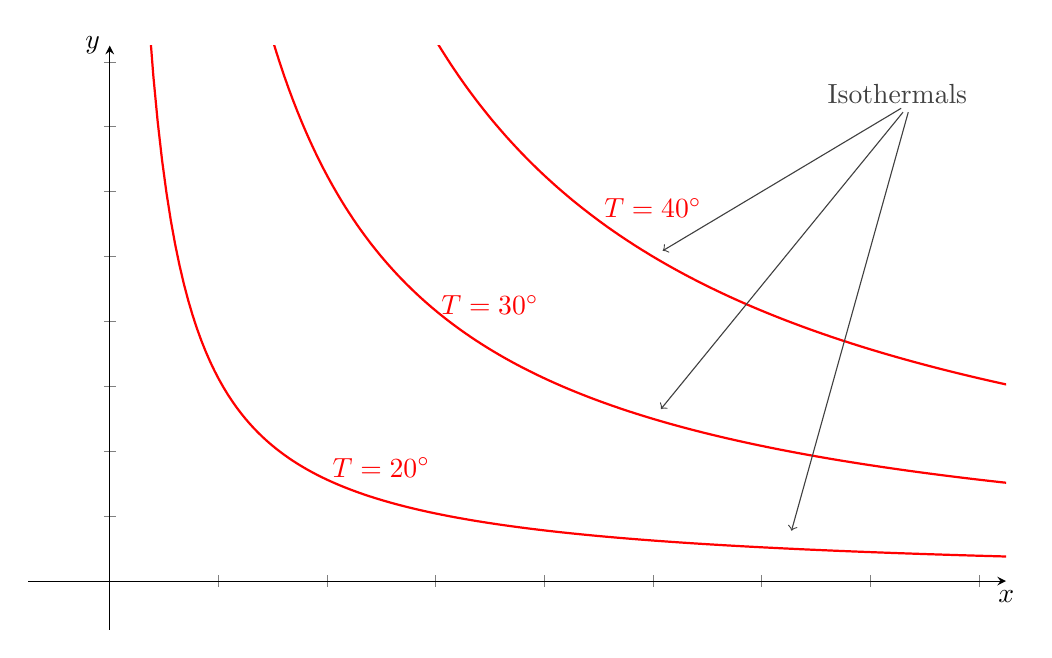
\begin{tikzpicture}
    \begin{axis}[
        legend pos=south east,
        axis x line=middle,
        axis y line=middle,
	every axis x label/.style={at={(current axis.right of origin)},anchor=north},
	every axis y label/.style={at={(current axis.above origin)},anchor=east},
	xticklabels=\empty,
	yticklabels=\empty
        grid = none ,
        width=14cm,
        height=9cm,
        grid style={dashed, gray!1},
        xmin=0,     % start the diagram at this x-coordinate
        xmax=1.5,    % end   the diagram at this x-coordinate
        ymin=0,     % start the diagram at this y-coordinate
        ymax=1.5,   % end   the diagram at this y-coordinate
        xlabel=$x$,
        ylabel=$y$,
        enlargelimits=true,
        tension=0.08]


         \addplot[domain=0:2, red,samples=250, thick] {1/(8*x)};
          \addplot[domain=0:2, red,samples=250, thick] {1/(2*x)};
           \addplot[domain=0:2, red,samples=250, thick] {1/(x)};
         \node(T1)[red] at (axis cs: 0.5, 0.35){$T= 20^{\circ}$};
         \node(T2)[red] at (axis cs: 0.7, 0.85){$T= 30^{\circ}$};
         \node(T3)[red] at (axis cs: 1,1.15){$T= 40^{\circ}$};
         \node(T3)[darkgray] at (axis cs: 1.45,1.5){Isothermals};
         
         \node(I0)  at (axis cs: 1.475, 1.475){};
         \node(I1)  at (axis cs: 1, 1){};
         \node(I2)  at (axis cs: 1, 0.5){};
         \node(I3)  at (axis cs:1.25,0.125){};
         
          \draw [darkgray, ->] (I0) -- (I1);
          \draw [darkgray,->] (I0) -- (I2);
          \draw [darkgray,->] (I0) -- (I3);
         
   
    \end{axis}
\end{tikzpicture}
\end{document}